\documentclass[11pt]{article}
\usepackage{graphicx}
\usepackage{float}
\usepackage{subfig}
\usepackage[margin=1in]{geometry}
\usepackage{amsmath}

\begin{document}

\section{Introduction}
This report presents the most relevant data quality issues found in the data set available for the project Improving the Effectiveness of Smart Work Zone Technologies (R27-155). This data set was generated and provided by two traffic management systems deployed by the company Ver-Mac.

\subsection{Setting}
A critical part of the project implementation is the development of realistic traffic micro-simulation models. Two work zones were chosen for simulation:
\begin{enumerate}
	\item \textbf{I-57/I-64:} IDOT Contract No. 78276, in Jefferson County, IL. 25 sensors were deployed; 22 radar sensors and 3 Remote Traffic Microwave Sensors (RTMS).
	\item \textbf{I-80:} IDOT Contract No. 60Y64, in Will County, IL. 30 sensors were deployed; 18 radar sensors and 12 RTMS. 
\end{enumerate}

\subsection{Data Set}
The data set of each work zone was accessed through the computer program JamLogic. The following data categories were required in 5 minute intervals:
\begin{itemize}
	\item Date and time
	\item Vehicle speed
	\item Vehicle count
\end{itemize}
The computer program JamLogic was used to export all of the available data as MS Excel spreadsheets. The spreadsheets were in turn converted into csv files and read by our data extraction code. This code has the capability of working with user specified sets of sensors and time intervals to:
\begin{itemize}
	\item Plot the correspondent data
	\item Export new csv files in a format that could be read by a traffic micro simulation program
\end{itemize}
 

\section{Methodology}
This section presents the procedures undertaken for assessing the quality of the data set.

\subsection{Preliminary Analysis}
The preliminary analysis of the data set was graphical. During the selection of appropriate modeling days, speed and count data were plotted. This had multiple purposes:
\begin{itemize}
	\item Identifying days with enough traffic congestion (needed for research purposes)
	\item Verifying data completeness
	\item Identifying other data abnormalities
\end{itemize}

\subsubsection{I-57/I-64}
From the plots generated, it was evident that the data set for this work zone had significant data incompleteness issues. The general trend was that when severe congestion occurred, the radar sensors would start having abnormal readings. An example of this is shown in figures \ref{fig:I-57/I-64 Missing Counts} and \ref{fig:I-57/I-64 Missing Speeds}:

\begin{figure}[H]
  \centering
  \subfloat[Vehicle count drops to zero in radar sensors.]{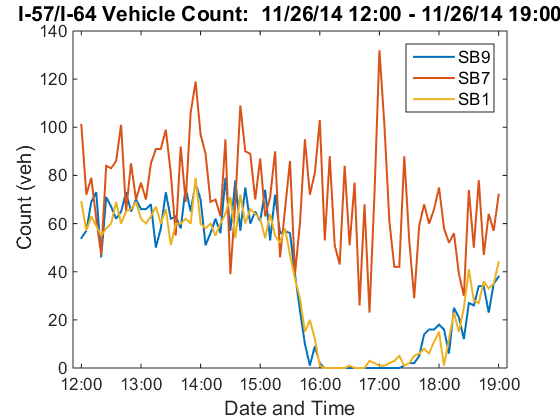
\includegraphics[width=0.46\textwidth]{Images/I57I64_missing_counts.png}\label{fig:I-57/I-64 Missing Counts}}
  \hfill
  \subfloat[Vehicle speed starts missing in radar sensors.]{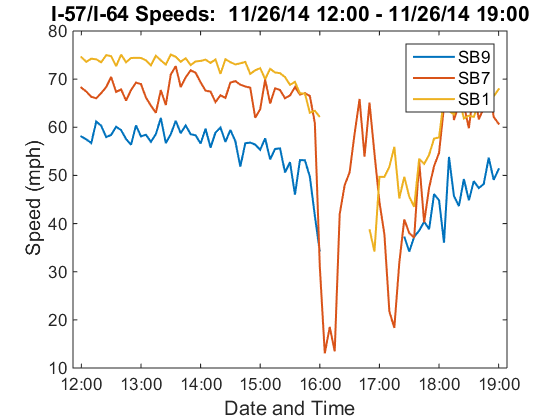
\includegraphics[width=0.46\textwidth]{Images/I57I64_missing_speeds.png}\label{fig:I-57/I-64 Missing Speeds}}
  \caption{Radar sensors present abnormal readings as traffic congestion starts.}
\end{figure}

\noindent
As shown above, sensors SB9 and SB1 (radar) presented the described issue, but SB7 (RTMS) did not. This situation was repeated for all of the remaining sensors in the work zone; radar sensors had the problem, but not the RTMS. This inconsistency made unclear which sensors were correct.



\subsubsection{I-80}
This work zone had serious issues with data inconsistency between sensors of different types. Specifically, sensors in a continuous section of road with no entrance or exit ramps presented significantly different readings. An example of this is shown in figures \ref{fig:I-80 Inconsistent Counts 1} and \ref{fig:I-80 Inconsistent Speeds 1}:

\begin{figure}[H]
  \centering
  \subfloat[Inconsistent vehicle counts.]{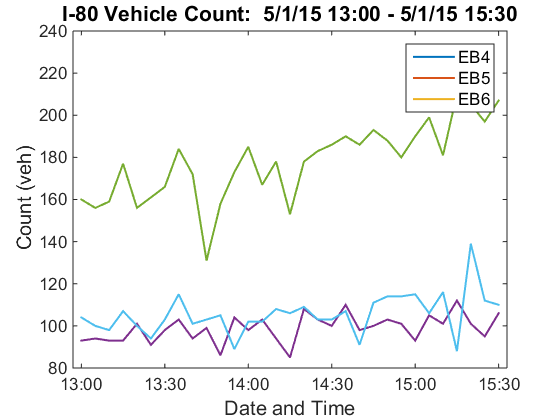
\includegraphics[width=0.46\textwidth]{Images/I80_inconsistent_counts_1.png}\label{fig:I-80 Inconsistent Counts 1}}
  \hfill
  \subfloat[Inconsistent vehicle speeds.]{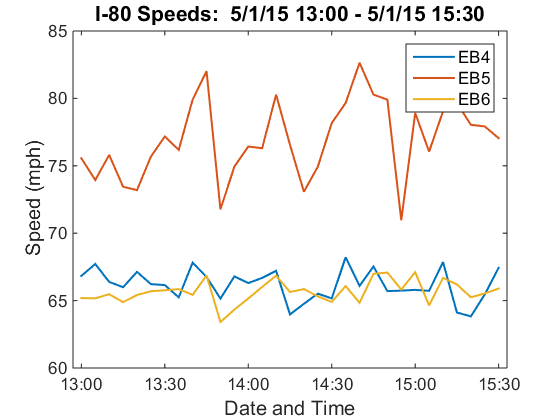
\includegraphics[width=0.46\textwidth]{Images/I80_inconsistent_speeds_1.png}\label{fig:I-80 Inconsistent Speeds 1}}
  \caption{Inconsistency between sensors EB4 and EB6 (radar) and EB5 (RTMS) during free flow.}
\end{figure}
\noindent
In general, RTMS sensors had greater readings for both speed and count. This violates mass conservation, meaning that at least one of the sensor types is presenting incorrect values.
 

\subsection{Full Scale Analysis}

\subsubsection{Description}
The statistical analysis performed for this data set is rather simple, but provides a good insight of the quality of the data. This section describes the procedures executed with the Python code provided.

\begin{description}
	\item[Arithmetic mean] \hfill \\
	The arithmetic means of data (speed or count) were determined for continuous user specified time intervals. The next equation was followed:	
	

	\begin{equation}
		\bar{x} = \frac{1}{n}\sum\limits_{i=1}^{n}x_i
		%\text{where~$R$ is Racoon,~$E$ is Elephant}
		\qquad\parbox{4.0cm}{\footnotesize$
		\begin{aligned}
			 n &= \text{ Number of time intervals}\\[-1.0ex]
			 x_{i} &= \text{ Sensor reading at time interval i}
		\end{aligned}$}
	\end{equation}	
	
	
	\item[Percent missing] \hfill \\
	The percents of missing data (speed or count) were determined for continuous user specified time intervals. The next equation was followed:

	\begin{equation}
		{Percent\:missing} = \frac{No.\:of\:missing\:readings}{No.\:of\:time\:intervals}*100	
	\end{equation}		
	
	\item[Percent change] \hfill \\
	The percents of change between the readings (speed or count) of two sensors were determined for used specified sensors and time intervals. The next equation was followed:
	
	\begin{equation}
		{Percent\:change\:(x_{f},x_{o})} = \frac{x_{f}-x_{o}}{x_{o}}*100
		\qquad\parbox{4.0cm}{\footnotesize$
		\begin{aligned}
			 x_{f} &= \text{ Reading from final sensor}\\[-1.0ex]
			 x_{o} &= \text{ Reading from initial sensor }
		\end{aligned}$}
	\end{equation}

\end{description}

\subsubsection{Findings}
This section presents the numerical results of the quality assessment procedures performed the data sets of each of the work zones. Note that both of the data sets used for this analysis were extracted in 5 minute intervals.
\begin{description}
	\item[I-57/I-64] \hfill \\
		\begin{itemize}
			\item Severe congestion was registered on November 26th, 2014. This can be confirmed by the lowering speeds shown in figure \ref{fig:I-57/I-64 Missing Speeds} and the corroboration from the engineers that were on site. Unfortunately, as it is evident from figures \ref{fig:I-57/I-64 Missing Counts} and \ref{fig:I-57/I-64 Missing Speeds}, great portions of data were missing. It was found that the radar sensors in the south bound direction missed an average (among the 8 radar sensors in this direction) of XX\% of the vehicle counts and XX\% of the vehicle speeds between XX:XX PM and XX:XX PM. The gaps of missing data were larger as the sensors approached the construction zone; during the same time interval, SB1 (upstream-most sensor) missed XX\% of the count data and XX\% of the speed data, while SB9 missed XX\% and XX\% of the data in the same order. This can be attributed to a longer duration of congestion near the interchange.
			
		\end{itemize}
	
	\item[I-80] \hfill \\
		\begin{itemize}
			\item  The readings (speed and count) of the RTMS sensors tended to be greater than those of the radar sensors. In May 2015, the RTMS sensors deployed on the east bound direction averaged XX mph and XX vehicles counted (per time step). On the other hand, the radar sensors averaged XX mph and XX vehicles counted.
		\\
		
Elaborating on this issue, averages of the percent differences between the readings of user specified pairs of sensors were found. The sensors chosen for this procedure were pairs of neighboring sensors on continuous segments of road with no entrances or exit ramps. It was found that, in May 2015, sensor EBX (RTMS) measured on average, XX\% higher speeds and counted XX\% more vehicles than its inmediate predecessor sensor EBX (radar). In the same circumstances, sensor EBX (RTMS) presented XX\% higher speeds and XX\% more vehicles than its immediate predecessor EBX (radar).

			\item There were a few cases of severe missing data issues. This issue was mainly isolated; specific sensors malfunctioned for a period of time, but the entirety of the system was never compromised. A specific case is that of sensor EBX (TYPE), which missed XX\% of the data in May 2015.
			
		\end{itemize}
\end{description}


\section{Conclusion}
The systematic issues present in each of the work zones made the determination of the sensors' accuracy problematic. In the case of I-57/I-64, there is no way to interpolate with sufficient certainty the large gaps of missing data. This means that the exact traffic behaviors at those  time intervals remain unknown. In the case of I-80, since both of the sensor types had relatively precise readings, it is troublesome to discern which one had correct measurements (or at least readings that were closer to reality). In fact, if not for the obvious violation of the principle of mass conservation, it would have been hard to identify the presence of the systematic errors in first place. Arriving to these conclusions would have been more arduous if all of the sensors had been placed next to entrance or exit ramps, for example.
\\
\\
The findings presented in this report are of importance for the three parties involved. IDOT may want to ensure that the sensors produce accurate readings. This would result in more reliable traffic estimations, which translates into an increased user safety. Ver-Mac may want to identify the sources of the odd sensor behaviors, so as to improve the quality of their traffic management systems and collaborate with IDOT's objectives. Our research group found it challenging to deal with the issues presented and had to implement creative solutions to move our project forward.


\end{document}